
% vim:fileencoding=utf-8:foldmethod=marker:foldmarker=(((,)))

% --- PÁGINA 8: CONTRAPORTADA ---

% === RAMAS CEREXZO === (((
\begin{figure}[h]
    \raggedleft
    \vspace{1.3cm} % <-- Baja la imagen la distancia que quieras
    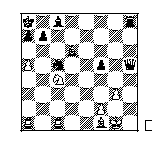
\includegraphics[width=0.5\linewidth]{pages/08-back-page/images/chess.pdf}\hspace*{-1.8cm}
    \label{fig:placeholder}
    \vspace{-1.3cm} % <-- ¡TRUCO! Cancela el espacio para que lo de abajo NO se mueva
\end{figure}
\noindent
\raisebox{-4.7cm}[0pt][0pt]{%
\hspace*{-2cm}\reflectbox{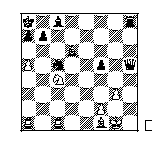
\includegraphics[width=0.5\linewidth]{pages/08-back-page/images/chess.pdf}}%
}
\vspace{-3.3cm}
% )))

% === CHESS PROBLEM === (((
\begin{center}
	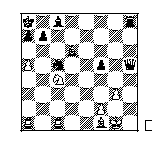
\includegraphics[width= 0.35 \linewidth, page = 1]{pages/08-back-page/images/chess.pdf}
\end{center}
\vspace{-0.4cm}
\begin{center}
	{\footnotesize\textbf{Mate en 7}}
\end{center}
\vspace{0.1cm}
% )))

% === PARTICIPANTS === (((
\begin{tcolorbox}[
    colback=white,          % Fondo blanco
    colframe=black,   
    boxrule=0.2mm,          % Borde negro
    arc=0mm,                % Esquinas rectas (sin redondeado)
    width=0.7\textwidth,    % Ajusta el ancho del rectángulo según lo necesites
    halign=center,          % Centra el contenido dentro de la caja
    valign=center,
    center                  % Centra la caja misma en la página
]
    {\large\textbf{Escritores Invitados}}
    \vspace{0.2cm}

    \footnotesize

		{\tt
		\begin{tabular}{r @{\hspace{2mm}} l}
			Lógica & Luis Martínez Aguilar \\ 
			& Sofía Espinasa Diamant \\ 
			& Diego Israel  \\ 
			& Serafín Adame 
		\end{tabular}
		}
    
\end{tcolorbox}
\vspace{0.1cm}
% )))

% === EDITORS === (((
\begin{tcolorbox}[
    colback=white,          % Fondo blanco
    colframe=black,   
     boxrule=0.2mm,    % Borde negro
    arc=0mm,                % Esquinas rectas (sin redondeado)
    width=0.7\textwidth,    % Ajusta el ancho del rectángulo según lo necesites
    halign=center,          % Centra el contenido dentro de la caja
    valign=center,
    center                  % Centra la caja misma en la página
]
    {\large\textbf{¿Te interesa colaborar?}}
    \vspace{0.2cm}

    
    \footnotesize
    {Editores}
    
    \vspace{0.1cm}
    {\textit{Yves Stanislas Ramírez Jiménez}}
    
    \vspace{0.1cm}
    {\textit{Ernesto Valerio }}

    \vspace{0.1cm}
    {\textit{Erick Rodríguez Juárez }}
\end{tcolorbox}
% )))
